\section{Sign languages}
\paragraph{}
\ac{sl} is one of the methods of communication, which is defined as a set of visual symbols or gestures that are used in a very systematic way for words, concepts, or ideas of a language "\cite{teaching}.
\paragraph{}
Despite the complexity of sign languages, they can be broken down into smaller units, such as signs, hand shapes, and movements. Sign languages typically use a combination of these units to form words and sentences. For example, \ac{asp} uses hand shapes, movements, and facial expressions to convey meaning.
\paragraph{}
Sign languages are not just visual representations of spoken languages, they are unique and independent languages with their syntax, grammar, and vocabulary. Recognizing and understanding them is therefore crucial for effective communication between hearing and deaf communities. In recent years, there has been increasing interest in developing technology to aid sign language recognition and translation.
\subsection{Most sign languages used in the world}
\paragraph{}
Around 5\% of the world population are deaf mute people "\cite{5perc}, they use different \ac{sl}s as their communication languages. that make a variety of \ac{sl}s used in the world. In table \ref{tab:major-sign-languages-of-the-world} we introduce the most used \ac{sl}s in the world.
\begin{table}[h]
	\caption{Major sign languages of the world "\cite{5perc}}
	\label{tab:major-sign-languages-of-the-world}
	\begin{tabular}{|l|l|c|}
		\hline
		\textbf{Country}  & \textbf{Sign Language} & \textbf{Abbn} \\
		\hline
		United Kingdom & British Sign Language & BSL \\
		\hline
		United States of America & American Sign Language & ASL \\
		\hline
		Commonwealth of Australia & Australian Sign Language & Auslan \\
		\hline
		Japan & Japanese Sign Language & JSL \\
		\hline
		People's Republic of China & Chinese Sign Language & CSL \\
		\hline
		Taiwan & Taiwanese Sign Language & TSL \\
		\hline
		Middle-East & Arabic Sign Language & ArSL \\
		\hline
		Islamic Republic of Iran and other Gulf countries & Persian Sign Language & PSL \\
		\hline
		Republic of India & Indian Sign Language & ISL \\
		\hline
		Republic of Turkiye & Turkish Sign Language & TSM \\
		\hline
		Republic of Kazakhstan & Kazakh-Russian Sign Language & K-RSL \\
		\hline
	\end{tabular}
\end{table}
\subsection{Sign languages in Algeria}
\paragraph{}
In Algeria, there is more than 240,000 deaf mute people "\cite{ethnologue}. However there was no official \ac{sl} for the country until 2002, when the Algerian government  recognized the \ac{asp} as official \ac{sl} in Algeria "\cite{wiki}. But this language is not the only one the country, there is also \ac{ajs}, an old \ac{sl} which eveloped in several Jewish communities is the region of M'zab, Algeria, which is located in the northern part of the Sahara desert "\cite{sara}.
\paragraph{}
For \ac{asp}, there is no official document or reference except for a dictionary published recently by the Algerian government. It contains some signs used by the deaf and other signs borrowed from the old \ac{fsl} "\cite{chalenges}. This book consists of illustrations for gestures organized in categories like religion, justice, education, etc. If the gesture require hand movements, they support the illustration with arrows to show the direction of the movement.
\subsection{Algerian Sign Language}
\paragraph{}
\ac{asp} is an \ac{sl} derived from \ac{fsl}, used by the deaf/mute community of Algeria. It was officially recognized by the Algerian law as official \ac{sl} in Algeria in May 2002 "\cite{wiki}. Technically, it is a visual-gestural language that uses hand shapes, movements, and facial expressions to convey meaning. Therefore, this community is often excluded from basic communication, this has caused many deaf Algerians to go without access to education, employment opportunities, and other basic rights. For that, The government of Algeria opened many deaf schools around the country to teach them the language itself, and basic education like any normal person.
\paragraph{}
Even with the existence of deaf schools, the teachers themselves are not qualified neither master \ac{asp}, all of them are hearing individuals who hold different degrees which are not related to deaf education or \ac{sl}, and they have never been trained to use the language before they get hired, some teachers attend training courses to learn alphabet only. And this makes it difficult for those pupils to get basic education and go even to middle or high school and college, most of them are marginalized and can only be manual workers, they are denied access to a high-quality education that meets their special needs to improve their lives and live as equal to their peers "\cite{chalenges}.
\begin{figure}[h]
	\centering
	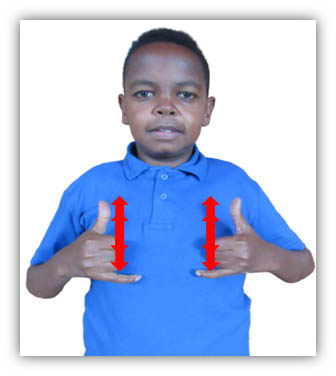
\includegraphics[width=0.8\linewidth]{images/AlgerianSignLanguage}
	\caption{Algerian Sign Language "\cite{asp_img}}
	\label{fig:algeriansignlanguage}
\end{figure}